\section{Detecting Cowrie Honeypots}

\begin{frame}{Introduction}
    \begin{columns}[T]
        % Column 1
        \begin{column}{0.5\textwidth}
            \begin{center}
                \enquote{Bad guys}\\
                Trying to detect honeypots
            \end{center}
        \end{column}
        % Column 2
        \begin{column}{0.5\textwidth}
            \begin{center}
                \enquote{Good guys}\\
                Trying to disguise honeypots
            \end{center}
        \end{column}
    \end{columns}
\end{frame}

\begin{frame}{Introduction}
    \begin{block}{\citet{vetterl2020}}
        There is a generic weakness in the current generation of low- and medium-interaction honeypots
    \end{block}
\end{frame}

\begin{frame}{Introduction}
    \begin{center}
        Can we detect honeypots?\footnote{Restrict to the SSH honeypot Cowrie}
    \end{center}
    \begin{center}
        OpenSSH $\leftrightarrow$ Cowrie
    \end{center}
\end{frame}

\begin{frame}{OpenSSH}
    \begin{figure}
        \centering
        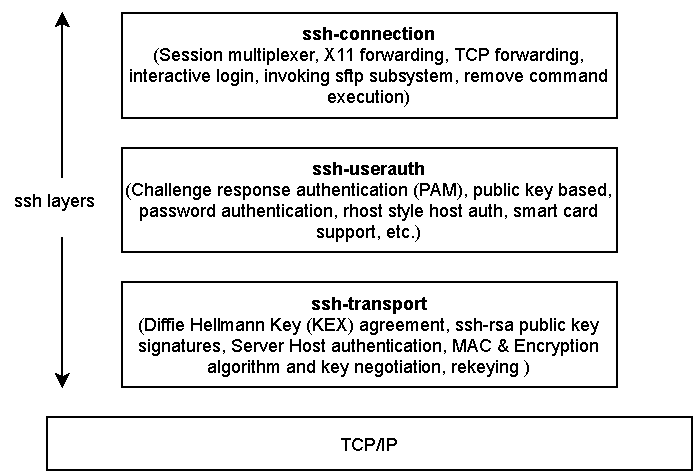
\includegraphics[width=0.9\columnwidth]{img/openssh-architecture.pdf}
        \caption[OpenSSH architecture]{
            OpenSSH's architecture (derived from \cite{openssh2007})
        }
    \end{figure}
\end{frame}

\begin{frame}{Cowrie}
    \begin{columns}
        % Column 1
        \begin{column}{0.3\textwidth}
            SSH and Telnet Honeypot
        \end{column}
        % Column 2
        \begin{column}{0.7\textwidth}
            \begin{figure}
                \centering
                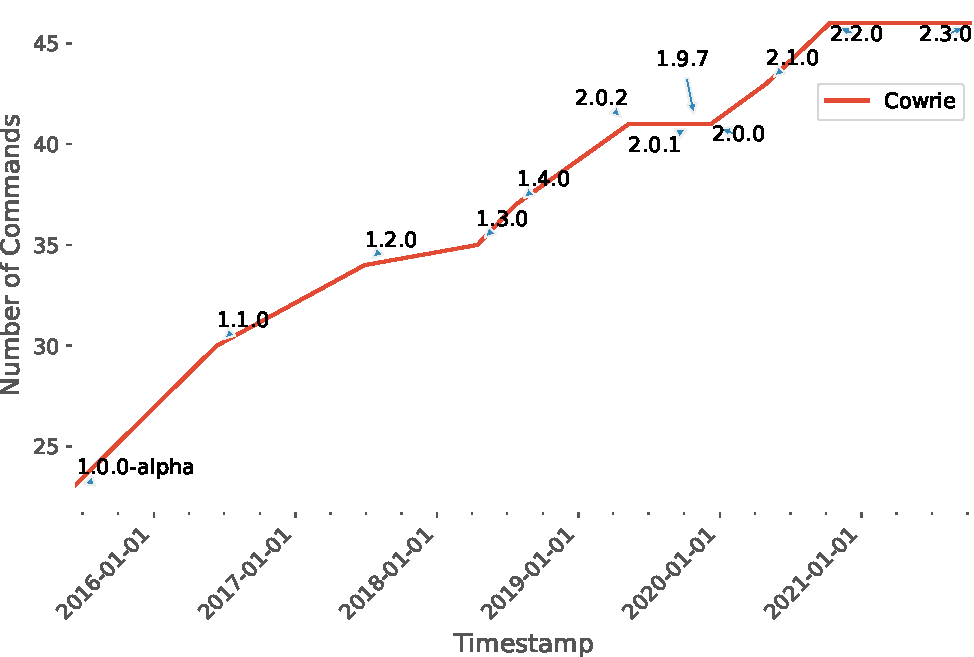
\includegraphics[width=\columnwidth]{img/cowrie-cmd.pdf}
                \caption[Cowrie commands]{
                    Number of Cowrie commands.
                }
            \end{figure}
        \end{column}
    \end{columns}
\end{frame}

\begin{frame}{How do we implement honeypots}
    \begin{columns}[T]
        % Column 1
        \begin{column}{0.5\textwidth}
                \begin{enumerate}
                \item Find a library for the protocol
                \item Write a program that is \enquote{just like bash}
                \item Adapt messages to be \enquote{just like OpenSSH}
            \end{enumerate}
        \end{column}
        % Column 2
        \begin{column}{0.5\textwidth}
            \begin{figure}
                \centering
                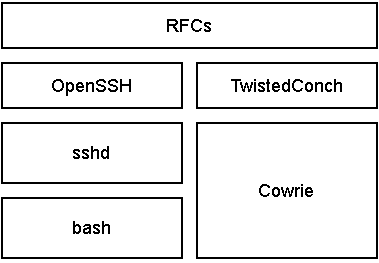
\includegraphics[width=0.6\columnwidth]{img/cowrie-openssh.pdf}
                \caption[Architecture of OpenSSH and Cowrie]{
                    Architecture of OpenSSH and Cowrie (derived from \cite{vetterl2020}.
                }
            \end{figure}
        \end{column}
    \end{columns}
    \vfill
    \begin{center}
        Problem $\rightarrow$ subtle differences between OpenSSH and Cowrie
    \end{center}
\end{frame}

\begin{frame}{Fingerprint Honeypots}
    \begin{columns}
        % Column 1
        \begin{column}{0.5\textwidth}
            \begin{figure}
                \centering
                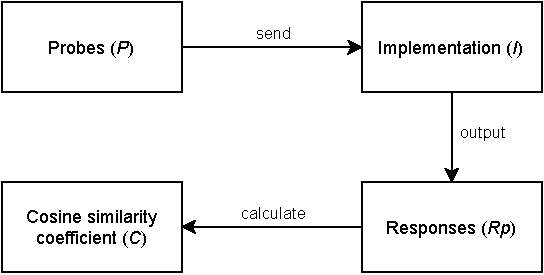
\includegraphics[width=\columnwidth]{img/vetterl_concept.pdf}
            \end{figure}
        \end{column}
        % Column 2
        \begin{column}{0.5\textwidth}
            \begin{itemize}
                \item \numprint{192} SSH version strings (RFC4253)
                \item \numprint{58752} SSH2\_MSG\_KEXINIT (RFC4250)
            \end{itemize}
        \end{column}
    \end{columns}
    \vfill
    SSH version string \enquote{SSH-2.2-OpenSSH \textbackslash r \textbackslash n}
    
    SSH2\_MSG\_KEXINIT
    {\footnotesize
    \begin{itemize}
        \item \textit{ecdh-sha2-nistp521} as the key-exchange algorithm
        \item \textit{ssh-dss} as host key algorithm
        \item \textit{blowfish-cbc} as encryption algorithm
        \item \textit{hmac-sha1} as mac algorithm
        \item \textit{zlib@openssh.com} as compression algorithm
    \end{itemize}
    }
    $\rightarrow$ resulting in the lowest cosine similarity coefficient $C$.
\end{frame}

\begin{frame}{Vetterl's findings}
    % cosine sim
    \begin{table}
        \caption{Cosine similarity of OpenSSH, Cowrie, and Twisted}
        \begin{tabular}{l|ccccc}
            \toprule
            OpenSSH & 6.6 & 6.7 & 6.8 & 7.2 & 7.5\\
            \hline
            Cowrie & $0.78$ & $0.79$ & $0.79$ & $0.79$ & $0.78$\\
            Twisted & $0.41$ & $0.41$ & $0.42$ & $0.42$ & $0.42$\\
            \bottomrule
        \end{tabular}
    \end{table}

\end{frame}

% Screenshot terminal
\begin{frame}{Reproduction}
    \begin{itemize}
        \item Adaption of custom SSH2\_MSG\_KEXINIT and String Version message
        \begin{itemize}
            \item OpenSSH: successful connection
            \item Cowrie: bad packet length exception
        \end{itemize}
    \end{itemize}
    $\rightarrow$ Underlying bug in TwistedConch
\end{frame}

\begin{frame}{Disguise Cowrie}
    \begin{columns}
        % Column 1
        \begin{column}{0.3\textwidth}
            Packets flow through OpenSSH
        \end{column}
        % Column 2
        \begin{column}{0.7\textwidth}
            \begin{figure}
                \centering
                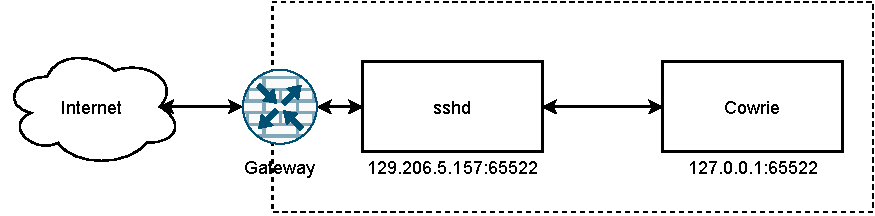
\includegraphics[width=\columnwidth]{img/sshd-honeypot.pdf}
                %\caption[Architecture of OpenSSH and Cowrie]{
                %    Architecture of OpenSSH and Cowrie (derived from \cite{vetterl2020}).
                %}
            \end{figure}
        \end{column}
    \end{columns}
\end{frame}

\begin{frame}{Experiment}
Latest OpenSSH version with latest Cowrie version
    \begin{itemize}
        \item Packets are received by Cowrie through OpenSSH
        \item No exception occurred
    \end{itemize}
\end{frame}

\begin{frame}{Summary}
    \begin{itemize}
        \item Reproduced Vetterl's findings
        \begin{itemize}
            \item Detecting honeypots on the transport level remains feasible
            \item It is easy to use scripts in tools such as \textit{Metasploit}
        \end{itemize}
        \item Updated Vetterl's method to work with the latest versions
        \item Disguised Cowrie to avoid such activities
    \end{itemize}
\end{frame}